\documentclass[conference]{IEEEtran}
%\documentclass[journal,compsoc]{IEEEtran}
\usepackage{graphics}
\usepackage{amsfonts}
\usepackage{wasysym}
\usepackage{listings}



% correct bad hyphenation here
\hyphenation{op-tical net-works semi-conduc-tor}


\begin{document}
%
% paper title
% can use linebreaks \\ within to get better formatting as desired
\title{Private Anonymous Messaging With Friends}


% author names and affiliations
% use a multiple column layout for up to three different
% affiliations
\author{\IEEEauthorblockN{Ruchith Fernando}
\IEEEauthorblockA{Department of Computer Science, Purdue University\\
West Lafayette, IN\\
rfernand@cs.purdue.edu}}





% make the title area
\maketitle


\begin{abstract}
%\boldmath
We identify a set of requirements in broadcasting messages among a set of trusted peers. Then we propose a scheme for contacts of a peer to obtain broadcast updates of the peer using a pull mechanism where the contacts' identities are maintained anonymous. 
We propose a modification to the hierarchical identity based encryption scheme proposed by Boneh et. al \cite{BBG05} where a peer can request and obtain messages of a common peer from another peer while remaining anonymous. We provide details of an implementation of the cryptographic primitives we propose as a prof of concept. \footnote {This work was done as a part of the course work of CS 626 : Advanced Information Assurance by Professor Cristina Nita-Rotaru}
\\
\end{abstract}

Keywords: Privacy, Peer-to-peer messaging, hierarchical identity based encryption


\IEEEpeerreviewmaketitle



\section{Introduction}

Today, social media is has become an integral part of day-to-day life. This includes services such as online social networks, micro blogging services etc. Furthermore, we have already seen the power of such tools in situations such as broadcasting opinions. This automatically leads way to censorship and suppression by political forces. Such control is feasible due to the current architecture of these services where they primarily adopt a client-server model. It is interesting to see different approaches in which we can maintain the power of social media while being able to resist control by third parties.

In this work we consider a peer-to-peer setup where the peers are \emph{only} connected to other peers who they personally trust. These are called $contacts$ of a peer. A peer distributes a message to its contacts (which we call an $update$) and all the peers are expected to receive this update. A peer may directly communicate the message when a contact is available online. We address the problem where there is only a sub set of contacts available to a peer to directly communicate a message and the other peers needs to obtain this message from those who have already possess it without compromising their privacy. We present a novel cryptographic approach as a solution to this problem.

Following section introduces the setup of the network of peers and how they are connected and the requirements that we try to satisfy with our scheme. This is followed by the preliminary notions and then we describe our solution that meets the stated requirements. Implementation of the proposed cryptographic primitives is presented in the solution section followed by future directions of this work and conclusion.


\section{Problem}


\subsection{Background}
A peer in this system is a user who has a set of other peers registered with it as contacts. This peer registration is bi-directional. In other words when peer A becomes a contact of peer B, peer B becomes a contact of peer A. 

A peer intends to send messages to all its contacts. All of these messages are to be delivered to the peer's contacts at that point of time. This is similar to the notion of microblogging. (Example: Twitter\cite{twitter}). Such a message is identified as an $update$.

We demote the a peer generating an $update$ as $P$ and its contacts as the set $C = \{C_{P_i}\}$ where $i \in \{1 , ..., n\}$ where $n$ is the number of contacts of $P$.

\subsection{Requirements}
We identify the following requirements in distributing messages in the above system.
\begin{itemize}
	\item A peer $P$ should be able to simply send its $update$ $M_P$ only to those contacts who are available online at the point of time it sends the update using direct connections to those peers. We denote the set of online contacts as  ${C^+} \subseteq C$ where $|{C^+}| \geq 1$.
	\item Those other contacts of $P$ who were off-line at when $P$ sent $M_P$ should be able to obtain $M_P$ when they are available online. We denote these contacts as ${C^-} \subset C$.
	\item Any $C_{P_i} \in C^-$ will be able to publish a query requesting an update of $P$. This is called an update request and is denoted by $Q_P$.
	\item Any  $C_{P_i} \in C^+$ will be able to publish a response to a $Q_P$. This response is denoted by $S_P$ and an eavesdropper with polynomially bounded resources should not be able to compute the original $M_P$ using $S_P$.
	\item The contact who provides $S_P$ should not be able to learn who generated $Q_P$.
	\item The contact who generates $Q_P$ and receives the corresponding $S_P$ should not be able to learn who generated $S_P$.
	\item When the composition of $C$ changes to new set of peers $C'$, $P$ should be able to update private configuration of the members of $C'$ with the issue of a public message.
	\item After such an update those peers in the set $C - C'$ should not be able to obtain an $update$ of $P$.
\end{itemize}
The scheme we propose in section IV addresses all these requirements.

For example consider figure~\ref{fig:fig1}. In this situation Alice is $P$. Alice has four contacts: Bob, Charlie, David and Nancy, out of which only Bob gets the $update$ $M_P$. Therefore: $C = \{Bob, Charlie, David,Nancy\}$, ${C^+ = \{Bob\}}$ and ${C^- = \{Charlie, David,Nancy\}}$. 

Note that a peer only trusts and has knowledge of its immediate contacts and is not aware of connections between those peers and their contacts. There are practical implementations of the notion of friend-only networks such as Freenet/Darknet \cite{darknet} and GNUnet \cite{gnunet}. We only consider cryptography related aspects of the solution to the identified problem in this work.

\begin{center}
\begin{figure}[here]
\resizebox{!}{6cm}{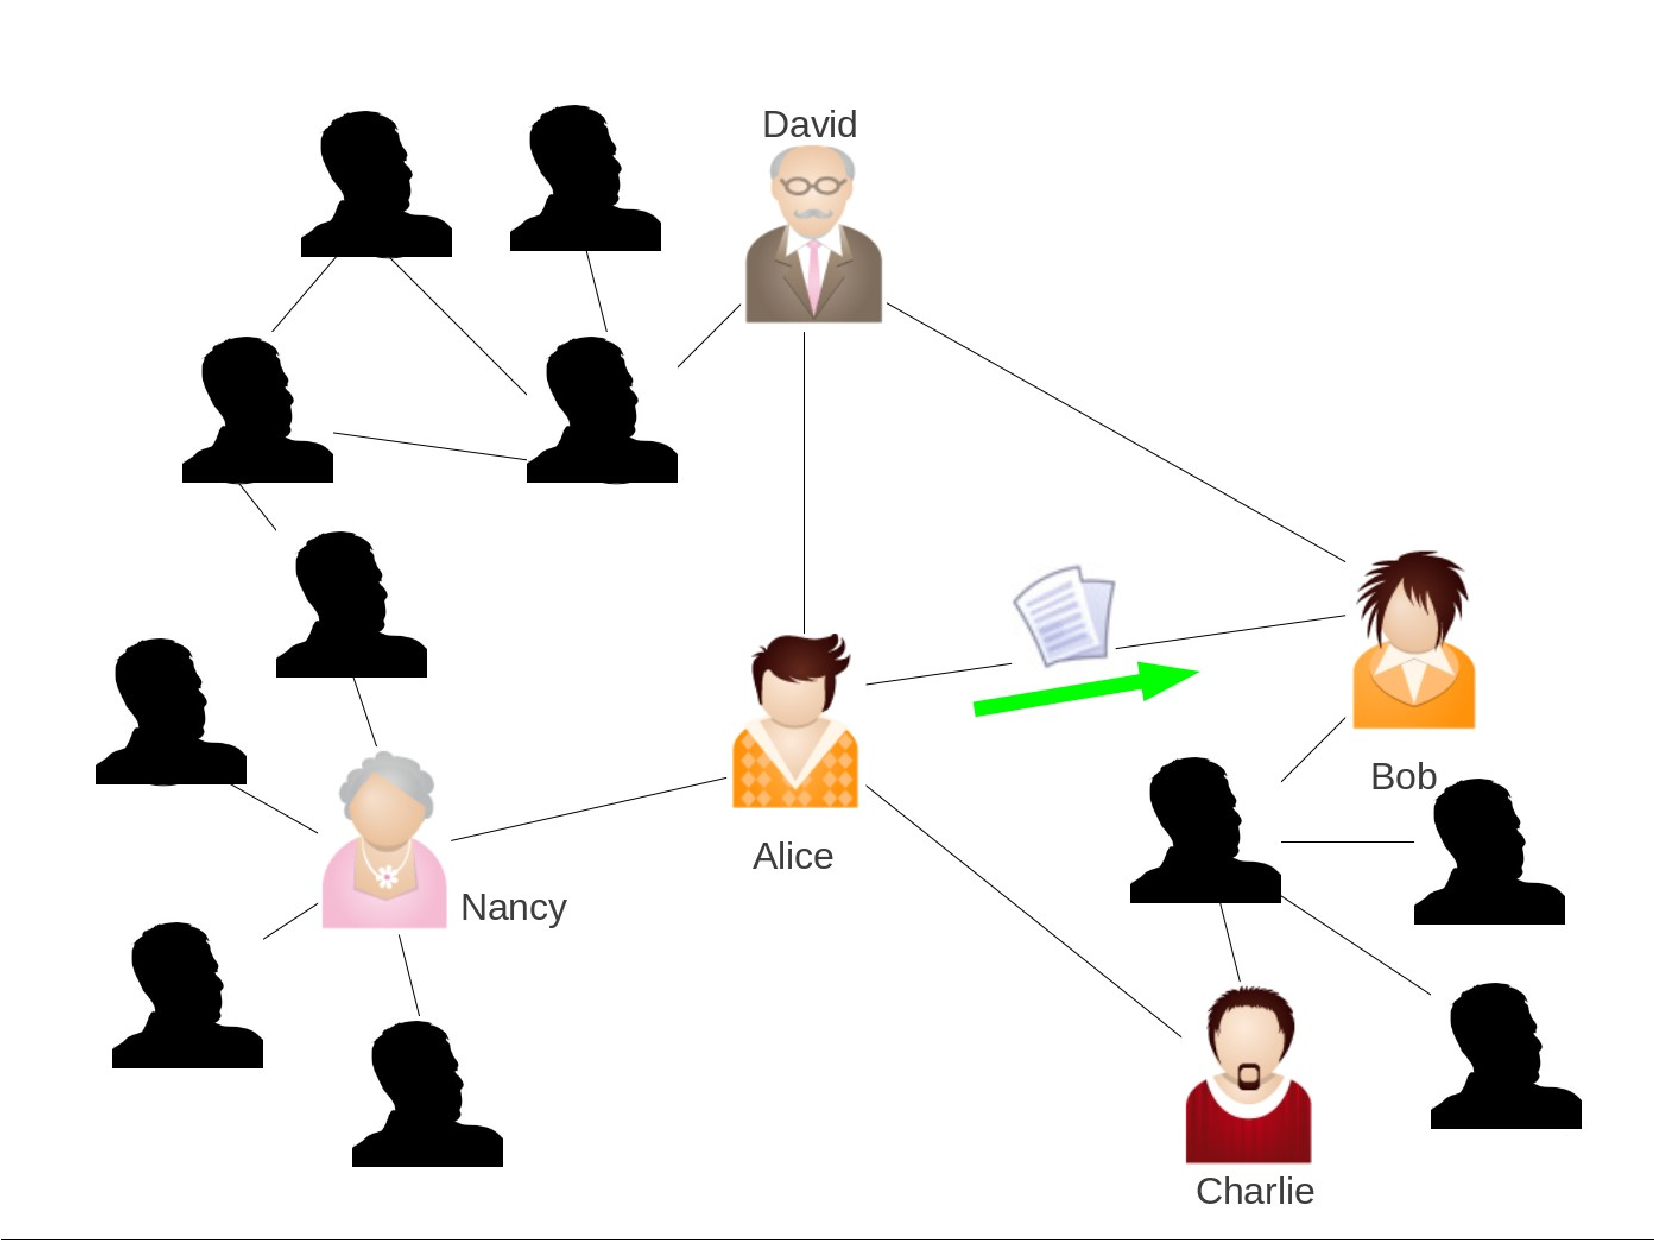
\includegraphics{img/img1.pdf}}
\caption{A user (Alice) and her contacts (Bob, Charlie, David and Nancy)}
\label{fig:fig1}
\end{figure}
\end{center}


\section{Preliminary Notions}

In this section we introduce the necessary background information that our work is based on.

\subsection{Hierarchical Identity Based Encryption (HIBE)}
Identity based encryption first proposed by Shamir\cite{Shamir:1985:ICS:19478.19483} is a public key encryption scheme where the identity of an entity can be used as the public key. The first complete solution for this was presented by Boneh and Franklin \cite{Boneh:2003:IEW:639069.639089}. Any party who intends to send a message to another will simply use a set of public parameters of a trusted authority along with the identity of the recipient will encrypt using this scheme. The recipient of the cipher text will be able to obtain the corresponding private key from the third party (who executes private key generation algorithm for the given identity after authenticating the requester) and decrypt the cipher text to obtain the plain text.

This idea of identity based encryption was extended to a hierarchy of identities \cite{Horwitz02towardhierarchical}, \cite{BBG05}, where at each level the private key is used as the input to the key generation algorithm along with the global parameters defined by the root. The HIBE system is defined in \cite{BBG05} as follows (which we modify in deriving out scheme):\\

Let $e : \mathbb{G} \times \mathbb{G} \to \mathbb{G}_1 $ be a bilinear map where $\mathbb{G}$ is a group of prime order $p$. An identity is defined as $ID = (I_1, ..., I_k) \in ({{\mathbb{Z}}^*}_p)^k$ where $k$ is the depth of the hierarchy that the $ID$ belongs to.

There are four algorithms: $Setup$, $KeyGen$, $Encrypt$ and $Decrypt$. $l$ is the maximum depth of the hierarchy allowed.\\

\begin{itemize}
\item $Setup (l)$, generates the public parameters and the master key as follows:
\begin{itemize}
	\item Select a generator $g \in \mathbb{G}$ and a random $\alpha \in \mathbb{Z}_p$
	\item Set $g_1 = g^{\alpha}$
	\item Pick random $g_2, g_3, h_1, ..., h_l \in \mathbb{G}$
	\item $params = (g, g_1, g_2, g_3, h_1, ..., h_l)$
	\item $master-key = {g_2}^{\alpha}$\\
\end{itemize}	

\item $KeyGen(d_{{ID}_{k-1}}, ID)$, generates the private key of the given $k^{th}$ level $ID$ using a $k-1$ level private key ($k \leq l$).

First suppose the $k-1$ level private key was generated using the master key :
\begin{itemize}
	\item Select a random $r \in \mathbb{Z}_p$ 
	\item Output $d_{{ID}_{k-1}}$ : \\
	$({{g_2}^{\alpha}} \cdot {({{h_1}^{I_1}\cdot \cdot \cdot {h_{k-1}}^{I_{k-1}}} \cdot {g_3} )}^r , g^r, {h_{k}}^r, ... , {h_l}^r) = (a_0, a_1, b_k, ... , b_l)$
\end{itemize}	

Now the $k^{th}$ level private key:
\begin{itemize}
	\item Select a random $t \in \mathbb{Z}_p$ 
	\item Output $d_{{ID}_{k}}$ : \\
	$({{a_0}\cdot{{b_k}^{I_k}}} \cdot {({{h_1}^{I_1}\cdot \cdot \cdot {h_k}^{I_k}} \cdot {g_3} )}^t , {a_1}\cdot{g^t}, {h_{k+1}}^t, ... , {h_l}^t)$\\
\end{itemize}	

\item $Encrypt (params, ID, M)$, encrypts a message $M \in \mathbb{G}$ using the public key $ID = (I_1, ..., I_k)$ :

\begin{itemize}
	\item Select a random $s \in \mathbb{Z}_p$ 
	\item Output $CT$ : \\
	$(e(g_1, g_2)^s \cdot M,  g^s,  {({{h_1}^{I_1}\cdot \cdot \cdot {h_k}^{I_k}} \cdot {g_3} )}^s)$\\$=(A, B, C)$\\
\end{itemize}	


\item $Decrypt (d_{ID}, CT)$, decrypts a given cipher text of the above form $(A, B, C)$ using the given private key of the form $(a_0, a_1, b_k, ... , b_l)$. \\
$(A \cdot e(a_1, C))/(e(B, a_0)) = M$\\
\end{itemize}

Next section describes how this scheme is used to meet the requirements identified in section II.


\section{Proposed Solution}

Here we present the scheme that addresses the requirements identified in section II. We discuss the details of setting up the parameters of a peer, registering contacts, contacts generating update requests to be processed by other contacts, update response to such a request and re-key of the system at a peer and how contacts update themselves.

\subsection{Peer Setup}
A peer $P$ will have a two level HIBE system parameters. This is by calling $setup(2)$.
This will generate generates the public parameters and the master key of the peer as follows:
\begin{itemize}
	\item Select a generator $g \in \mathbb{G}$ and a random $\alpha \in \mathbb{Z}_p$
	\item Set $g_1 = g^{\alpha}$
	\item Pick random $g_2, g_3, h_1, h_2 \in \mathbb{G}$
	\item $params = (g, g_1, g_2, g_3, h_1, h_2)$
	\item $master-key = {g_2}^{\alpha}$
\end{itemize}


\subsection{Registering a Contact}

The main idea is to setup a two level ($l=2$) HIBE system at each peer. When a peer $P$ registers a $C_{P_i}$ it will create a new random first level identifier $I_{r_i} \in \mathbb{Z}_p$ and corresponding private key ($d_{I_{r_i}}$). The private key and the identifier will be communicated to $C_{P_i}$ using a private channel. $d_{I_{r_i}}$ is of the form
$({{g_2}^{\alpha}} \cdot {({{h_1}^{I_{r_i}}} \cdot {g_3} )}^r , g^r, {h_2}^r)$ ,
where $r \in \mathbb{G}$ is random.

\begin{itemize}
\item $C_{P_i}$ keeps both $I_{r_1}$ and $d_{I_{r_1}}$ private along with the public parameters of $P$
\item $P$ stores the tuple $<I_{r_i}, r>$, \footnote {This is used to update contact parameters in the case of a re-key.}
\end{itemize}


\subsection{A Contact Requesting an Update}
When $P$ sends an $update$ message it may send the update directly to available contacts by encrypting the message using their corresponding identifiers. The interesting case is when a contact $C_{P_{req}}$ needs to obtain the latest $update$ of $P$ and $P$ is no longer available online. In such a situation, as highlighted by in the requirements, $C_{P_{req}}$ will be able to generate a request for $P$'s update, $Q_p$. This is generated as follows:

Suppose the identifier assigned to $C_{P_{req}}$ by $P$ is $I_{r_1}$
\begin{itemize}
\item Select a random $I_{r_2}\in \mathbb{Z}_p$
\item Set $ID_{req} = {h_1}^{I_{r_1}} \cdot {h_2}^{I_{r_2}}$
\item Update Request to be published $Q_P = <P, ID_{req}>$, here $P$ is an identifier string of $P$ known to all $P$'s contacts.
\end{itemize}

$C_{P_{req}}$ publishes $<P, ID_{req}>$ and any of $P$'s other contacts will be able to respond to this request. This request information can simply be made publicly available using a common medium. The steps in creating the response is described next.

\subsection{Encryption and Update Response}
When a contact of $P$ observes the tuple $<P, ID_{req}>$ and decides to serve this request it will first encrypt the latest $update$ message $M_P$ from $P$ using the following modified encryption function ($Encrypt'$) and $P$'s public parameters $params_P$. 

$Encrypt' (params_P, ID_{req}, M_P)$ :

\begin{itemize}
	\item Select a random $s \in \mathbb{Z}_p$ 
	\item $CT_{resp} = (e(g_1, g_2)^s \cdot M,  g^s,  {({ID_{req}} \cdot {g_3})}^s) = (A, B, C)$
\end{itemize}

The contact can now publish the tuple \\$<P, ID_{req}, CT_{resp}>$ as the response $S_P$.

\subsection{Decryption of the Update}
The contact that generated the update request will obtain the response available and do the following to obtain the plain update message $M_P$. Now it can generate the corresponding private key using the first level private key it possesses, using ${I_{r_2}}$ (used to generate $ID_{req}$) as the second level identifier. Suppose the first level private key is $d_{I_{r_1}} = (a_0, a_1, b_2)$, then:

\begin{itemize}
\item Private key for $ID_{req}$ : $d_{ID_{req}}$ 
\begin{center}
$= ({{a_0}\cdot{{b_2}^{I_{r_2}}}} \cdot {({{h_1}^{I_{r_1}}\cdot {h_2}^{I_{r_2}}} \cdot {g_3} )}^t , {a_1}\cdot{g^t})$\\
$ = ({a_0}', {a_1}')$\\\
\end{center}
\item Finally to decrypt $CT_{resp} = (A, B, C) $ :\\
	\begin{center}
$(A \cdot e({a_1}', C))/(e(B, {a_0}')) = M_P$\\\
	\end{center}
\end{itemize}


\subsection{Peer Re-key}
The set of contacts at a peer $C$ can change in two ways:
\begin{itemize}
\item When a new contact joins
\item when an existing contact is removed
\end{itemize}

When a new contact ($C_{P'}$) joins the peer $P$ simply can carryout new contact registration without and this doesn't require any changes to the parameters. The new contact will be able to request updates of the peer from its other contacts in the set ($C - C_{P'}$). 

However when $P$ needs to remove a contact $C_{P'}$ from the list of contacts, it has to update its parameters. We present an approach where we generate public information that the set $C - C_{P'}$ will be able to use to configure themselves.

In peer setup, the generated HIBE configuration if of the form  $params = (g, g_1, g_2, g_3, h_1, h_2)$ and $master-key = {g_2}^{\alpha}$ where $g_1 = g^{\alpha}$ and $\alpha \in \mathbb{Z}_p$ is random. In the case of re-key a peer :
\begin{itemize}
\item Generates a new random $\alpha' \in \mathbb{Z}_p$
\item Sets $master-key = {g_2}^{\alpha'}$
\item Set $g_1 = g^{\alpha'}$
\end{itemize}

With this change $P$ will have to update the private keys of the contacts. Note that in contact registration process $P$ stored the tuple $<I_{r_i}, r>$ for each contact $C_{P_i}$. 

To update contacts:

First generate a random $u \in \mathbb{Z}_p$

Initialize a list $<{id'}_i, A_i>$ and for each contact $C_{P_i} \in C$:
\begin{itemize}
\item generate the first component of the private keys of the contacts as ${{g_2}^{\alpha'}} \cdot {({{h_1}^{I_{r_i}}} \cdot {g_3} )}^{r_i} = A$. This $r$ value is from the stored $<I_{r_i}, r>$.
\item Add  $<{u^{I_{r_i}}}, A>$ to the $<{id'}_i, A_i>$ list.
\end{itemize}

Finally the complete re-key information to be published is 
\begin{center}
$<P, g_1, u, [<{id'}_1, A_1>, ...,  <{id'}_n, A_n>]>$ ,
\end{center} where $n = |C|$. Note that ${id'}_i$ is the identifier of $C_{P_i}$ blinded using $u$ where ${id'}_i = u^{I_{r_i}}$.\\

When a peer $C_{P_i} \in C$ obtains this information it will simply do the following :
\begin{itemize}
\item Update $P$'s public parameters by replacing the $g_1$ value with received value.
\item Retrieve its identifier issued by $P$ ($I_{r_i}$) and compute $id' = u^{I_{r_i}}$
\item Obtain the updated first component of its private key from the list $[<{id'}_1, A_1>, ...,  <{id'}_n, A_n>]$ using $id'$.\\
\end{itemize}

Evaluation section, discusses how this scheme meets the identified requirements.


\section{Evaluation}


\section{Implementation}
The proposed scheme was implemented in Java as a library using Java Pairing Based Cryptography \cite{jpbc} library. The demo application developed uses this library in to demonstrate the features of this library. This work available under LGPL at anon-encrypt project hosted in google code \cite{ae}.

\subsection{Library}
Talk about test cases also

\subsection{Demo application}






\section{Future Work}

TODO Add comparison with broadcast encryption somewhere\\

Reduce the re-key size\\
\subsection{Size of re-key information}
Currently we generate a minimum amount of information that is required to re-key a peer and its contacts. But in this scheme the re-key informaiton is of order n where n is the number of contacts of the peer. It would be interesting to evaluate the possibility of reducing the size of this public information while maintaining the same properties.

\subsection{Incentives to forward messages}
This sheme relies on the fact that the contacts belonging to the set $C^+$ (those who holds the latest $M_P$) will respond to an $update$ request $Q_P$ with correct a response $S_P$. It will be useful to evaluate the possibility of coming up with an incentive scheme for contacts in $C^+$ to respond to $Q_P$s.

\subsection{Security roof}
We plan to prove that an adversary with polynomially bounded resources will not be able to ...??

\subsection{Implementation of message routing}
The current implementation only covers the cryptographic primitives. It will be interesting to use these with a peer to peer network where the peers are connected only to their private contacts and evaluate the performance. It might be possible to be implemented as a plugin to Freenet \cite{freenet}.



\section{Conclusion}
We proposed the cryptographic primitives to address the problem of distributing a message from a common peer using a pull mechanism where the peers requesting the message can request messages anonymously. Details of the scheme was provided followed by a high level evaluation of security. As a proof of concept of the proposed cryptographic functionality, we developed an implementation and finally identified the possible future improvements and research related to this work.



\bibliographystyle{unsrt} 
\bibliography{ref}

\end{document}
